<+	+>	!comp!	!exe!
%        File: !comp!expand("%:p:t")!comp!
%     Created: !comp!strftime("%a %b %d %I:00 %p %Y ").substitute(strftime('%Z'), '\<\(\w\)\(\w*\)\>\(\W\|$\)', '\1', 'g')!comp!
% Last Change: !comp!strftime("%a %b %d %I:00 %p %Y ").substitute(strftime('%Z'), '\<\(\w\)\(\w*\)\>\(\W\|$\)', '\1', 'g')!comp!
%
\documentclass{article}
\usepackage{tikz}
\usetikzlibrary{mindmap,trees}
\tikzset{concept/.append style={fill={none}}}
\usepackage{enumerate}

\begin{document}
\pagestyle{empty}
\centering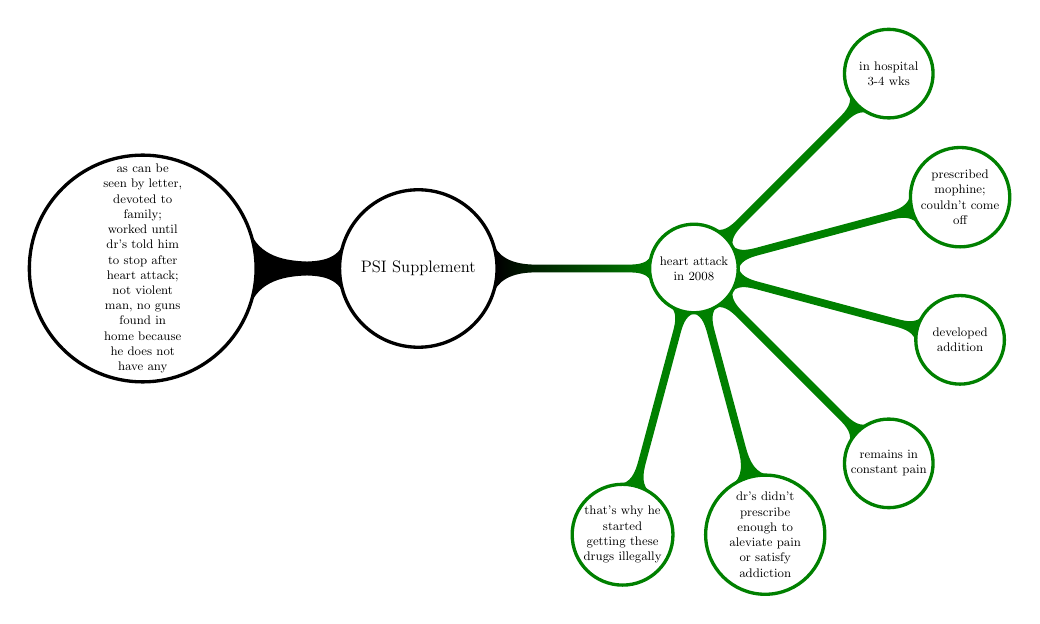
\begin{tikzpicture}[grow cyclic, text width=2.7cm, align=flush
  center, scale=0.50, transform shape]
\path[mindmap,concept color=black,text=black, grow cyclic, align=flush center, level
  1 concept/.append style={level distance=7cm,sibling
  angle=-180}, level
2/.style={level distance=7cm,sibling angle=30},
  ]
        node[concept] {PSI Supplement}
        [clockwise from=0]
        child[concept color=green!50!black] {
  node[concept] {heart attack in 2008}
        [clockwise from=45]
          child { node[concept] {in hospital 3-4 wks} }
          child { node[concept] {prescribed mophine; couldn't come off} }
          child { node[concept] {developed addition} }
          child { node[concept] {remains in constant pain} }
          child { node[concept] {dr's didn't prescribe enough to
  aleviate pain or satisfy addiction} }
          child { node[concept] {that's why he started getting these
  drugs illegally} } }
          child { node[concept] {as can be seen by letter, devoted to
  family; worked until dr's told him to stop after heart
  attack; not violent man, no guns found in home because he
  does not have any} 
  };
\end{tikzpicture}



\begin{enumerate}

\item 

\end{enumerate}

    \end{document}
